\label{sec:appendix_pac}
Given a model parameterized with $\theta$ and an input-label pair $(\vx,\vy)\in\R^d\times \R^c$, the classification error of $\theta$ over the input sample $\vx$ is $\breve{l}(\theta, \vx) := \1[\arg\max f_\theta(\vx) = \arg\max\vy].$ With the underlying data distribution $D$ and training set $S$ i.i.d. sampled from $D$, we define
\begin{equation}
e(\theta):=\E_{(\vx, \vy)\sim D}[\breve{l}(\theta,\vx)],\qquad \hat{e}(\theta):=\frac{1}{N}\sum_{i=1}^N[\breve{l}(\theta,\vx_i)]
\end{equation}
as the expected and empirical classification error of $\theta$, respectively.
We define the measurable hypothesis space of parameters $\gH:= \R^P$.
%\znote{measurability is STATEd for KL to be generally well-defined, do we need to define $P$ and $Q$ as probability measure as well?}
For any probabilistic measure $P$ in $\gH$, let $e(P) = \E_{\theta\sim P}e(\theta)$, $\hat{e}(P) = \E_{\theta\sim P}\hat{e}(\theta)$, and $\breve{e}(P) = \E_{\theta\sim P}\mathcal{L}(\theta)$. Here $\breve{e}(P)$ serves as a differentiable convex surrogate of $\hat{e}(P).$

\begin{theorem}[Pac-Bayes Bound]
\citep{mcallester1999some}\citep{langford2001bounds}
For any prior distribution $P$ in $\gH$ that is chosen independently from the training set $S$, and any posterior distribution $Q$ in $\gH$ whose choice may inference $S$, with probability $1-\delta$,
\begin{equation}
    \label{eqn:appendix_pac_bayes_inf}
    \KL\left(\hat{e}(Q)\Vert e(Q)\right)\leq \frac{\KL(Q\Vert P) + \log\frac{|S|}{\delta}}{|S|-1}.
\end{equation}
\end{theorem}
Fix some constant $b, c \geq 0$ and $\theta_0\in\gH$ as a random initialization, \citet{dziugaite2017computing} shows that when setting $Q = \gN(\vw, \diag(\vs))$, $P = \gN(\theta_0, \lambda\mI_P)$, where $\vw, \vs\in\gH$ and $\lambda = c\exp{(-j/ b)}$ for some $j\in\mathbb{N}$, and solve the optimization problem
\begin{equation}
    \min_{\vw,\vs,\lambda}\breve{e}(Q) + \sqrt{\frac{\KL(Q\Vert P) + \log\frac{|S|}{\delta}}{2(|S|-1)},}
\end{equation} with initialization $\vw = \theta$, $\vs = \theta^2$,
one can achieved a nonvacous PAC-Bayes bound by \equationref{eqn:appendix_pac_bayes_inf}.

In order to avoid discrete optimization for $j\in \N$, \citet{dziugaite2017computing} uses the $\BRE$ term to replace the bound in \tableref{eqn:appendix_pac_bayes_inf}. The $\BRE$ term is defined as
\begin{equation}
    \BRE(\vw,\vs,\lambda; \delta) = \frac{\KL(P\Vert Q)+2\log(b\log \frac{c}{\lambda})+\log \frac{\pi^2 |S|}{6\delta}} {|S|-1},
\end{equation}
where $Q = \gN(\vw, \diag(\vs))$, $P = \gN(\theta_0, \lambda\mI_P)$.
The optimization goal actually used in the implementation is thus
\begin{equation}
    \min_{\vw \in \R^P,\vs\in \R^P_+,\lambda\in (0,c)}\breve{e}(Q) + \sqrt{\frac{1}{2}\BRE(\vw,\vs,\lambda; \delta)}.
\end{equation}

\algorithmref{alg:pac} shows the algorithm for \emph{Iterative Hessian} (\textsc{Iter}) PAC-Bayes Optimization. If we set $\eta = T$, the algorithm will be come \emph{Approximate Hessian} (\textsc{Appr}) PAC-Bayes Optimization. It is based on Algorithm 1 in \citet{dziugaite2017computing}. The initialization of $\vw$ is different from \citet{dziugaite2017computing} because we believe what they wrote, $\abso(\vw)$ is a typo and $\log[\abso(\vw)]$ is what they actually means. It is more reasonable to initialize the variance $\vs$ as $\vw^2$ instead of $\exp[2\abso(\vw)]$.

\begin{algorithm}[ht]
\caption{PAC-Bayes bound optimization using layer-wise Hessian eigenbasis}
\textbf{Input:}\\
\algind$\vw_0\in\R^P$\Comment{Network parameters (Initialization)}\\
\algind$\vw\in \R^P$\Comment{Network parameters (SGD solution)}\\
\algind$S$ \Comment{Training examples}\\
\algind$\delta \in (0,1)$ \Comment{Confidence parameter}\\
\algind$b \in \mathbb{N}, c \in (0,1)$ \Comment{Precision and bound for $\lambda$}\\
\algind$\tau\in(0,1), T \in\mathbb{N}$ \Comment{Learning rate; No. of iterations}\\
\algind$\eta \in \mathbb{N}$ \Comment{Epoch interval for Hessian calculation}\\
\textbf{Output}\\
\algind$\vw$\Comment{Optimized network parameters}\\
\algind$\vs$\Comment{Optimized posterior variances in Hessian eigenbasis}\\
\algind$\lambda$\Comment{Optimized prior variancce}
\begin{algorithmic}[1]
\Procedure{Iterative-Hessian-PAC-Bayes}{}
    \State $\vvarsigma \gets \log[\abso(\vw)]$\Comment{where $\vs(\vvarsigma)= \exp(2\vvarsigma)$}
    \State $\varrho \gets -3$\Comment{where $\lambda(\varrho) = \exp(2\varrho)$}
    \State $R(\vw, \vs, \lambda) = \sqrt{\frac{1}{2}\BRE(\vw,\vs,\lambda; \delta)}$
    \Comment{BRE term}
    \State $B(\vw,\vs,\lambda,\vw') = \Ls(\vw')+R(\vw,\vs,\lambda)$\Comment{Optimization goal}
    \For{$t = 0 \to T-1$}\Comment{Run SGD for T iterations}
        \If{$t\mod \eta == 0$}
            \State $\textsc{HessianCalc}(w)$
        \EndIf
        \State \text{Sample} $\vxi \sim \N(0,1)^P$ 
        \State $\vw'(\vw,\vvarsigma)= \vw +\textsc{ToStandard}\left(\vxi \odot \exp(\vvarsigma)\right)$ \Comment{Generate noisy parameter for SNN}
        \State $\vw \gets \vw- \tau\left[\nabla_\vw R(\vw, \vs, \lambda)+\nabla_{\vw'}\Ls(\vw')\right]$
        \State $\vvarsigma \gets \vvarsigma - \tau\left[\nabla_\vvarsigma R(\vw, \vs(\vvarsigma), \lambda)+\textsc{ToHessian}\left(\nabla_{\vw'}\Ls(\vw')\right)\odot \vxi \odot \exp(\vvarsigma)\right]$
        \State $\varrho \gets \varrho - \tau\nabla_{\varrho}R(\vw,\vs,\lambda(\varrho))$ \Comment{Gradient descent}
    \EndFor
    \State \Return $w, s(\vvarsigma), \lambda(\varrho)$
\EndProcedure
\end{algorithmic}
\label{alg:pac}
\end{algorithm}

% \begin{algorithm2e}[ht]
% \caption{PAC-Bayes bound optimization using layer-wise Hessian eigenbasis}
% \SetKwInOut{KwInput}{Input}
% \SetKwInOut{KwOutput}{Output}
% \KwInput{
% $\vw_0\in\R^P$\tcp{Network parameters (Initialization)}
% $\vw\in \R^P$\tcp{Network parameters (SGD solution)}
% $S$ \tcp{Training examples}
% $\delta \in (0,1)$ \tcp{Confidence parameter}
% $b \in \mathbb{N}, c \in (0,1)$ \tcp{Precision and bound for $\lambda$}
% $\tau\in(0,1), T \in\mathbb{N}$ \tcp{Learning rate; No. of iterations}
% $\eta \in \mathbb{N}$ \tcp{Epoch interval for Hessian calculation}}
% \KwOutput{
% $\vw\in \R^P$\tcp{Optimized network parameters}
% $\vs\in \R^P$\tcp{Optimized posterior variances in Hessian eigenbasis}
% $\lambda \in \R_+$\tcp{Optimized prior variancce}}
% \Begin{
%     $\vvarsigma \gets \log[\abso(\vw)]$\tcp{where $\vs(\vvarsigma)= \exp(2\vvarsigma)$}
%     $\varrho \gets -3$\tcp{where $\lambda(\varrho) = \exp(2\varrho)$}
%     $R(\vw, \vs, \lambda) = \sqrt{\frac{1}{2}\BRE(\vw,\vs,\lambda; \delta)}$
%     \tcp{BRE term}
%     $B(\vw,\vs,\lambda,\vw') = \Ls(\vw')+R(\vw,\vs,\lambda)$\tcp{Optimization goal}
%     \For(\tcp*[h]{Run SGD for T iterations}){$t = 0 \to T-1$} {
%         \If{$t\mod \eta == 0$} {
%             $\textsc{HessianCalc}(w)$
%         }
%     Sample $\vxi \sim \N(0,1)^P$ 
%     $\vw'(\vw,\vvarsigma)= \vw +\textsc{ToStandard}\left(\vxi \odot \exp(\vvarsigma)\right)$ \tcp{Generate noisy parameter for SNN}
%     $\vw \gets \vw- \tau\left[\nabla_\vw R(\vw, \vs, \lambda)+\nabla_{\vw'}\Ls(\vw')\right]$\\
%     $\vvarsigma \gets \vvarsigma - \tau\left[\nabla_\vvarsigma R(\vw, \vs(\vvarsigma), \lambda)+\textsc{ToHessian}\left(\nabla_{\vw'}\Ls(\vw')\right)\odot \vxi \odot \exp(\vvarsigma)\right]$\\
%     $\varrho \gets \varrho - \tau\nabla_{\varrho}R(\vw,\vs,\lambda(\varrho))$ \tcp{Gradient descent}
%     }
%     \Return $w, s(\vvarsigma), \lambda(\varrho)$
% }\label{alg:pac}
% \end{algorithm2e}

In the algorithm, \textsc{HessianCalc}$(\vw)$ is the process to calculate Hessian information with respect to the posterior mean $\vw$ in order to produce the Hessian eigenbasis to perform the change of basis. For very small networks, we can calculate Hessian explicitly but it is prohibitive for most common networks. However, efficient approximate change of basis can be performed using our approximated layer-wise Hessians. In this case, we would just need to calculate the full eigenspace of $\E[\mM]$ and that of $\E[\vx\vx^\T]$ for each layer. For $p$th layer, we denote them as $\mU^{(p)}$ and $\mV^{(p)}$ respectively with eigenvectors as columns. We can also store the corresponding eigenvalues by doing pairwise multiplications between eigenvalues of $\E[\mM]$ and $\E[\vx\vx^\T]$.

After getting the eigenspaces, we can perform the change of basis. Note that we perform change of basis on vectors with the same dimensionality as the parameter vector (or the posterior mean). $\textsc{ToHessian}(\vu)$ is the process to put a vector $\vu$ in the standard basis to the Hessian eigenbasis. We first break $\vu$ into different layers and let $\vu^{(p)}$ be the vector for the $p$th layer. We then define $\Mat^{(p)}$ as the reshape of a vector to the shape of the parameter matrix $\mW^{(p)}$ of that layer. We have the new vector $\vv^{(p)}$ in Hessian basis as
\begin{equation}
\label{eqn:appendix_pacbayes_changebasis}
    \vv^{(p)} = \vect\left[\mU^{(p)T}\Mat^{(p)}(\vu^{(p)})\mV^{(p)}\right].
\end{equation}
The new vector $\vv = \textsc{ToHessian}(\vu)$ is thus the concatenation of all the $\vv^{(p)}$.

$\textsc{ToStandard}(\vv)$ is the process to put a vector $\vv$ in the Hessian eigenbasis to the standard basis. It is the reverse process to $\textsc{ToHessian}$. We also break $\vv$ into layers and let the vector for the $p$th layer be $\vv^{(p)}$. Then, the new vector $\vu^{(p)}$ is
\begin{equation}
    \vu^{(p)} = \vect\left[\mU^{(p)}\Mat^{(p)}(\vv^{(p)})\mV^{(p)T}\right],
\end{equation}
The new vector $\vu = \textsc{ToStandard}(\vv)$ is thus the concatenation of all $\vu^{(p)}$.

After getting optimized $\vw, \vs, \lambda$, we compute the final bound using Monte Carlo methods same as in \citet{dziugaite2017computing}.

Note that the prior $P$ is invariant with respect to the change of basis, since its covariance matrix is a multiple of identity $\lambda\mI_P$. Thus, the KL divergence can be calculate in the Hessian eigenbasis without changing the value of $\lambda$. In the \emph{Iterative Hessian with approximated output Hessian} (\textsc{Iter.M}), we use $\Tilde{M}$ to approximate $\E[\mM]$, as in \equationref{eqn:M_SAS_Approx}.

We followed the experiment setting proposed by \citet{dziugaite2017computing} in general. In all the results we present, we first trained the models from Gaussian random initialization $w_0$ to the initial posterior mean estimate $w$ using SGD (lr=0.01) with batch-size 128 and epoch number 1000.

We then optimize the posterior mean and variance with layer-wise Hessian information using \algorithmref{alg:pac},
where $\delta = 0.025$, $b=100$, and $c=0.1$.
We train for 2000 epochs, with learning rate $\tau$ initialized at 0.001 and decays with ratio 0.1 every 400 epochs. For \emph{Approximated Hessian} algorithm, we set $\eta=1$. For \emph{Iterative Hessian} algorithm, we set $\eta=10$. We also tried $\eta$ with the same decay schedule as learning rate (multiply $\eta$ by 10 every time the learning rate is multiplied by 0.1) and the results are similar to those without decay.
We also used the same Monte Carlo method as in \citet{dziugaite2017computing} to calculate the final PAC-Bayes bound. Except that we used 50000 iterations instead of 150000 iterations because extra iterations do not further tighten the bound significantly. We use sample frequency 100 and $\delta'=0.01$ as in that paper.

The complete experiment results are listed in \tableref{tab:app_pac}. We follow the same naming convention as in \citet{dziugaite2017computing} except adding T-$200^2$ we introduced in \sectionref{sec:hessian}. T-$600_{10}$, T-$600^2_{10}$, and T-$200^2_{10}$ are trained on standard MNIST with 10 classes, and others are trained on MNIST-2 (see \sectionref{sec:appendix_exp_dataset}), in which we combined class 0-4 and class 5-9.

In \tableref{tab:app_pac}, Prev means the previous results in \citet{dziugaite2017computing}, \textsc{Appr} means \emph{Approximated Hessian}, \textsc{Iter} means \emph{Iterative Hessian}, \textsc{Iter} (D) means \emph{Iterative Hessian} with decaying $\eta$, \textsc{Iter.M} means \emph{Iterative Hessian with approximated output Hessian}. \textsc{Base} are Base PAC-Bayes optimization as in the previous paper.

We also plotted the final posterior variance, $\vs$. \figureref{fig:app_PAC} shown below is for T-$200^2_{10}$. For posterior variance optimized with our algorithms (\textsc{Appr}, \textsc{Iter}, and \textsc{Iter.M}) we can see that direction associated with larger eigenvalue has a smaller variance. This agrees with our presumption that top eigenvectors are aligned with sharper directions and should have smaller variance after optimization. The effect is more significant and consistent for Iterative Hessian, where the PAC-Bayes bound is also tighter.
\begin{figure}[H]
    \centering
    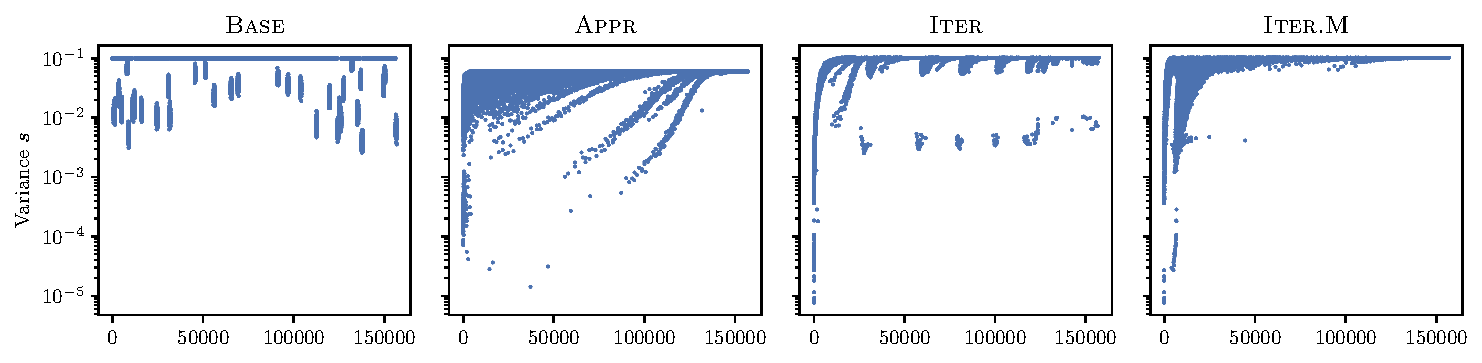
\includegraphics[width=\textwidth]{Figures/PacBayes/FC2_10cls/sigma_post_compare_iter_iterH_Sigma_post_MNIST_Exp1FC2_fixlr0.01_fc1.weight.pdf}
    % \captionsetup{justification=centering}
    \caption{Optimized posterior variance, $\vs$. (fc1:T-$200^2$, trained on MNIST), the horizontal axis is ordered with decreasing eigenvalues.}
    \label{fig:app_PAC}
\end{figure}

\newpage



\begin{table}[H]
  \centering
  \caption{Full PAC-Bayes bound optimization results}
  \vskip 0.1in
    \begin{center}
    \begin{tabular}{llccccc}
    \toprule
    \textbf{Network} & \textbf{Method} &  \shortstack{PAC-Bayes\\Bound} & \shortstack{KL\\Divergence} & \shortstack{SNN\\loss} & \shortstack{$\lambda$ (prior)} &\shortstack{Test\\Error} 
    \\ \midrule
    T-600          & \textsc{Prev}         & 0.161  & 5144   & 0.028   &    -    & 0.017 \\
                   & \textsc{Base}      & 0.154  & 4612.6 & 0.03373 & -1.3313 & 0.0153 \\
                   & \textsc{Appr}     & 0.1432 & 3980.6 & 0.03417 & -1.6063 & 0.0153 \\
                   & \textsc{Iter}       & \textbf{0.1198} & 3766.1 & 0.02347 & -1.2913 & 0.0153 \\
                   & \textsc{Iter(D)} & 0.1199 & 3751.1 & 0.02366 & -1.2913 & 0.0153 \\
                   & \textsc{Iter.M} & 0.1255 & 3929.9 & 0.02494 & -1.3213 & 0.0153\\
    \hline\rule{0pt}{2.5ex}
    T-$600^2$      & \textsc{Prev}        & 0.186  & 6534   & 0.028   &    -    & 0.016 \\
                   & \textsc{Base}      & 0.1921 & 6966.6 & 0.03262 & -1.4163 & 0.0148 \\
                   & \textsc{Appr}     & 0.1658 & 5176.1 & 0.03468 & -2.0963 & 0.0148 \\
                   & \textsc{Iter}       & 0.1456 & 5086.5 & 0.02473 & -1.7963 & 0.0148 \\
                   & \textsc{Iter(D)} & \textbf{0.1443} & 4956.8 & 0.02523 & -1.7963 & 0.0148 \\
                   & \textsc{Iter.M} & 0.1502 & 5024.5 & 0.02767 & -1.8363 & 0.0148\\
    \hline\rule{0pt}{2.5ex}
    
    
    T-1200         & \textsc{Prev}         & 0.179  & 5977   & 0.027   &    -    & 0.016 \\
                   & \textsc{Base}      & 0.1754 & 5917.6 & 0.03295 & -1.5463 & 0.0161 \\
                   & \textsc{Appr}     & 0.1725 & 5318.8 & 0.03701 & -1.8313 & 0.0161 \\
                   & \textsc{Iter}       & 0.1417 & 5071  & 0.02292 & -1.4763 & 0.0161 \\
                   & \textsc{Iter(D)} & \textbf{0.1413} & 5021.1 & 0.02316 & -1.4763 & 0.0161 \\
                   & \textsc{Iter.M} & 0.1493 & 5185.4 & 0.02576	& -1.5363 &	0.0161\\
    \hline\rule{0pt}{2.5ex}
    T-$300^2$      & \textsc{Prev}         & 0.17   & 5791   & 0.027   &    -    & 0.015 \\
                   & \textsc{Base}      & 0.1686 & 5514.9 & 0.03329 & -1.1513 & 0.015 \\
                   & \textsc{Appr}     & 0.1434 & 4105.4 & 0.03296 & -1.8063 & 0.015 \\
                   & \textsc{Iter}       & 0.1249 & 3873.2 & 0.02514 & -1.4763 & 0.015 \\
                   & \textsc{Iter(D)} & \textbf{0.1244} & 3833.7 & 0.02526 & -1.4763 & 0.015 \\
                   & \textsc{Iter.M} & 0.1308	& 3987.2 &	0.02721	 & -1.5713 & 0.015 \\
    \hline\rule{0pt}{2.5ex}
    R-600          & \textsc{Prev}         & 1.352  & 201131 & 0.112   &    -    & 0.501 \\
                   & \textsc{Base}      & 0.6046 & 1144.8 & 0.507   & -1.8263 & 0.4925 \\
                   & \textsc{Appr}     & 0.5653 & 390.25 & 0.5066  & -2.4713 & 0.4925 \\
                   & \textsc{Iter(D)} & 0.5681 & 431.62 & 0.5066  & -2.4513 & 0.4925 \\
                   & \textsc{Iter.M} & \textbf{0.5616} & 340.62 &	0.5065	& -2.5263 &	0.4925\\
    \hline\rule{0pt}{2.5ex}
    T-$200^2_{10}$     & \textsc{Base}      & 0.4165 & 21896  & 0.04706 & -1.1513 & 0.0208 \\
                   & \textsc{Appr}     & 0.2621 & 11068  & 0.0366  & -1.4213 & 0.0208 \\
                   & \textsc{Iter}       & \textbf{0.2145} & 9821  & 0.02229 & -1.1513 & 0.0208 \\
                   & \textsc{Iter(D)} & 0.2311 & 9758.5 & 0.03071 & -1.1513 & 0.0208 \\
                   & \textsc{Iter.M} & 0.2728 & 13406 & 0.02605	& -1.1513 &	0.0208\\
    \hline\rule{0pt}{2.5ex}
    T-$600_{10}$   & \textsc{Base}      & 0.2879 & 12674  & 0.03854 & -1.1513 & 0.018 \\
                   & \textsc{Appr}     & 0.2424 & 9095.8 & 0.04159 & -1.6013 & 0.018 \\
                   & \textsc{Iter}       & \textbf{0.2132} & 8697.9 & 0.02947 & -1.3063 & 0.018 \\
                   & \textsc{Iter.M} & 0.2227	& 8870.9	& 0.03294	& -1.4613	& 0.018 \\
    \hline\rule{0pt}{2.5ex}
    T-$600^2_{10}$ & \textsc{Base}      & 0.3472 & 17212  & 0.03884 & -1.1513 & 0.0186 \\
                   & \textsc{Appr}     & 0.2896 & 11618  & 0.04723 & -2.0563 & 0.0186 \\
                   & \textsc{Iter}       & \textbf{0.2431} & 10568 & 0.03057 & -1.5713 & 0.0186 \\
    \bottomrule
    \end{tabular}
\end{center}
  \label{tab:app_pac}
\end{table}
